\section*{Feature Selection}

Given a supervised learning task, feature selection is a process of selecting features s.t.\ the generalization performance of the predictive models is improved.

\textbf{Objectives:}
\begin{itemize}
    \item Avoid overfitting and improve generalization performance;
    \item Provide faster and more cost-effective models;
    \item Gain a deeper insight into the underlying processes that generated the data.
\end{itemize}

\begin{center}
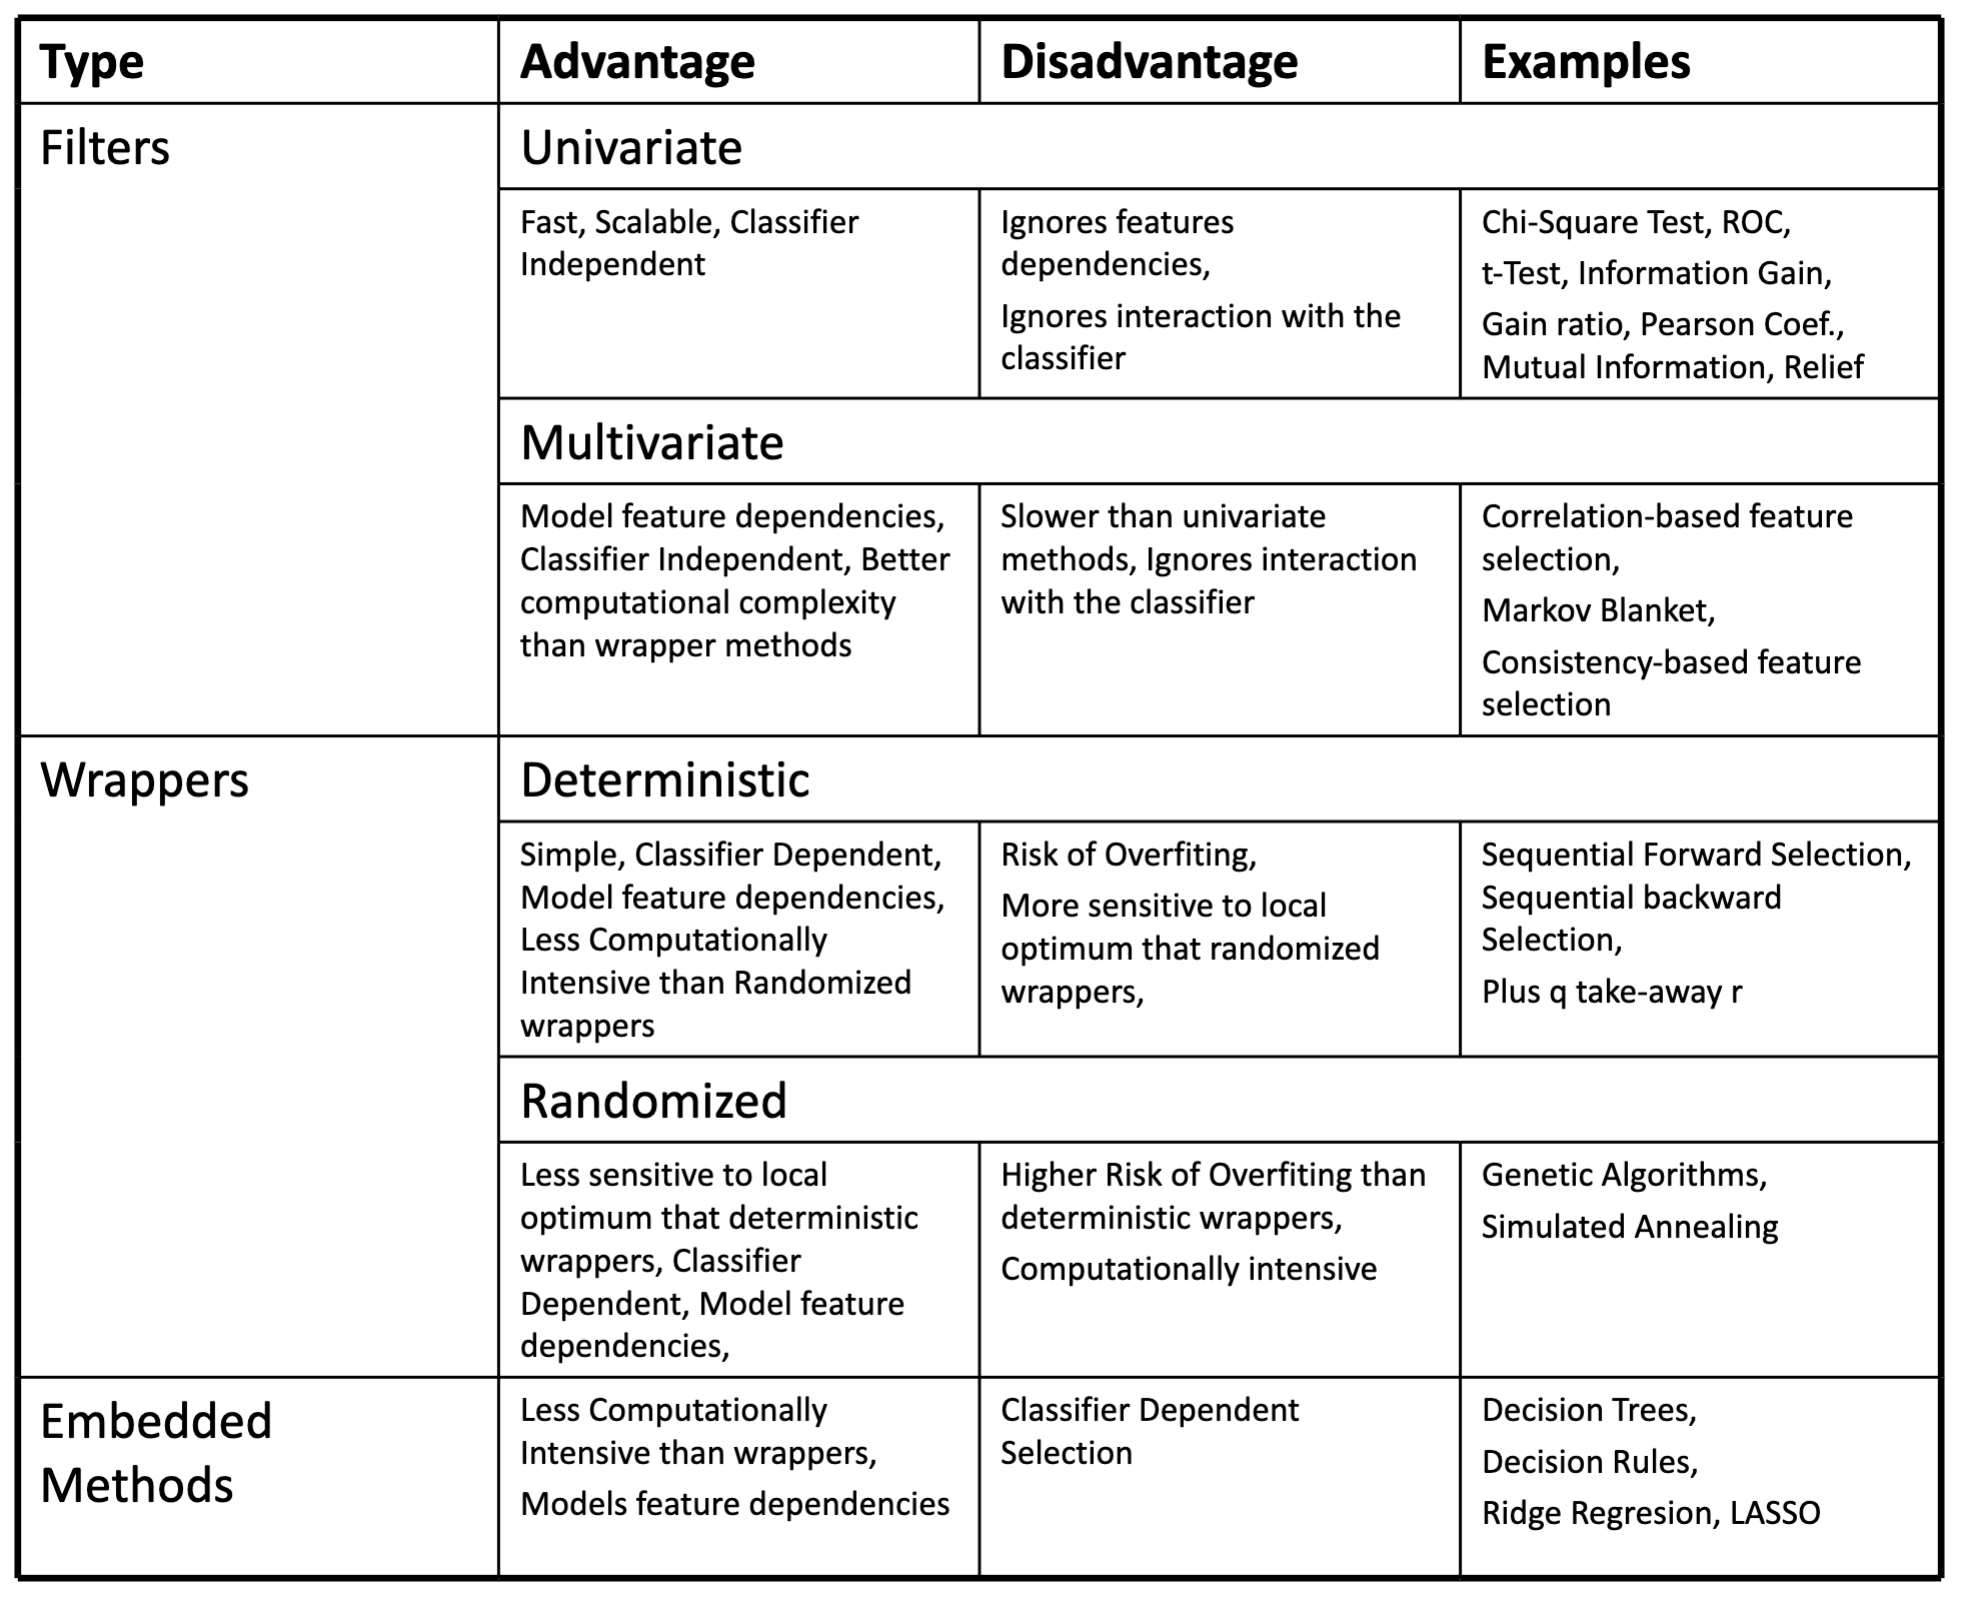
\includegraphics[width=0.8\textwidth]{images/image6.png}
\end{center}

\section*{Filters}
Rank features or feature subsets independently of the learning algorithm (classifier).

\begin{itemize}
    \item \textbf{Advantages:} Fast, Simple, Interpretable, Classifier independence, High dimensionality tolerance
    \item \textbf{Disadvantages:} Ignore interaction with classifiers, ignore feature dependencies.
\end{itemize}

\section*{Univariate Filters}

The relevance of individual feature $X_i$ is determined by how much $X_i$ can explain the output feature $Y$. Statistically this means that we need to assess the (in)dependence of $X_i$ and $Y$. In this context we have two questions:

1. Is $X_i$ independent of $Y$?
2. If $X_i$ and $Y$ are not independent, then how much are they dependent?

We have these scenarios:
\begin{itemize}
    \item The feature $X_i$ is discrete and the feature $Y$ is discrete: Chi-Square Test for Independence, ROC, Information gain and Ratio; Relief; Mutual Information.
    \item The feature $X_i$ is continuous and the feature $Y$ is discrete: t-Test on two means; Relief.
    \item The feature $X_i$ is continuous and the feature $Y$ is continuous: Mutual Information.
\end{itemize}

\section*{Multivariate Filters}
Multivariate Filters rank feature subsets independently on the type of the predictor later used. They operate by searching in the space of possible feature subsets and choosing those of subsets that maximize a given evaluation criterion.

$N$ features, $2^N$ possible feature subsets

\subsection*{Search}
\begin{itemize}
    \item \textbf{Search Direction:} Forward, Backward, Bidirectional
    \item \textbf{Search Strategy:} 
    \begin{itemize}
        \item Deterministic: Hill Climbing, Best First, Exhaustive
        \item Non-deterministic: Genetic
    \end{itemize}
\end{itemize}

\subsection*{Feature Subset Assessment}
Split the data into 3 subsets: training, validation, and test.
\begin{enumerate}
    \item For each feature subset, train predictor on training data.
    \item Select the feature subset which performs best on validation data.
    \item Repeat and average if you want to reduce variance (cross-validation).
    \item Test on test data.
\end{enumerate}

\subsection*{Data Leakage}
Data leakage in validation occurs when information from outside the training fold is used—directly or indirectly—during model training or preprocessing, causing the model to appear more accurate in evaluation than it really is.

\subsection*{Correlation Based Feature Selection}
Evaluation of feature subsets based on the next formula:

$$\text{CFS}(X_i, Y) = \frac{kr_{cf}}{\sqrt{k + (k-1)r_{ff}}}$$

where $S$ is a set with $k$ features, $r_{cf}$ is the average correlation between the features in $S$ and the class feature, and $r_{ff}$ is the average correlation between the features in $S$.

\section*{Wrappers}
Wrappers rank feature subsets w.r.t.\ the predictor used. They operate by searching in the space of possible feature subsets and choosing those of subsets that maximize a given evaluation criterion based on the predictor later used. The evaluation method of the classifier for feature evaluation usually is k-fold cross validation.

\subsection*{Recursive Feature Elimination}
Recursive Feature Elimination is a wrapper that recursively reduces the set of features by eliminating the least important ones based on the ranking provided by a specific model.

\begin{itemize}
    \item \textbf{Feature Dependency:} RFE takes into account the feature dependency assuming that are incorporated in the ranks.
    \item \textbf{Feature Ranking:} Not only does RFE help in selecting important features, but it also ranks all features based on their importance.
    \item \textbf{Handles Multicollinearity:} If some features are correlated, RFE can help in identifying and retaining the most important one among them.
    \item \textbf{Flexibility:} RFE can be used with any model that assigns weights or importance to features, making it versatile.
    \item \textbf{Computationally Intensive:} As RFE involves training the model multiple times (once for each feature), it can be computationally expensive.
    \item \textbf{Model Dependency:} The effectiveness of RFE is tied to the chosen model. A poorly chosen model might lead to sub-optimal feature selection.
    \item \textbf{Stability Issues:} Slight changes in the data can lead to different rankings, especially when features have similar importance.
    \item \textbf{Base Model Selection:} The choice of the model used in RFE is crucial. It's advisable to use a model that naturally provides importance or coefficient values, like decision trees, linear regression, or support vector machines.
\end{itemize}

\section*{Embedded Methods}
White box predictors are actually based on feature selection. So, embedded methods are all the learning algorithms that derive white box predictors. These include: Decision trees and rules, and Shrinkage methods such as ridge regression and LASSO.
